\documentclass[10pt,a4paper]{article}

\usepackage{fontspec}
\usepackage[top=1cm]{geometry}
\usepackage{graphicx}
\defaultfontfeatures{Mapping=tex-text}
\setromanfont[Ligatures={Common},Numbers={Lining}]{Linux Libertine}
\author{Michal Staniaszek}
\title{Answers to Question One}

\begin{document}
\maketitle

\begin{description}
\item[Alan] Studied his BSc in Electrical Engineering here at KTH and is now
  doing his second year in the Systems, Control and Robotics masters program,
  Robotics and Autonomous Systems track.
  \\
  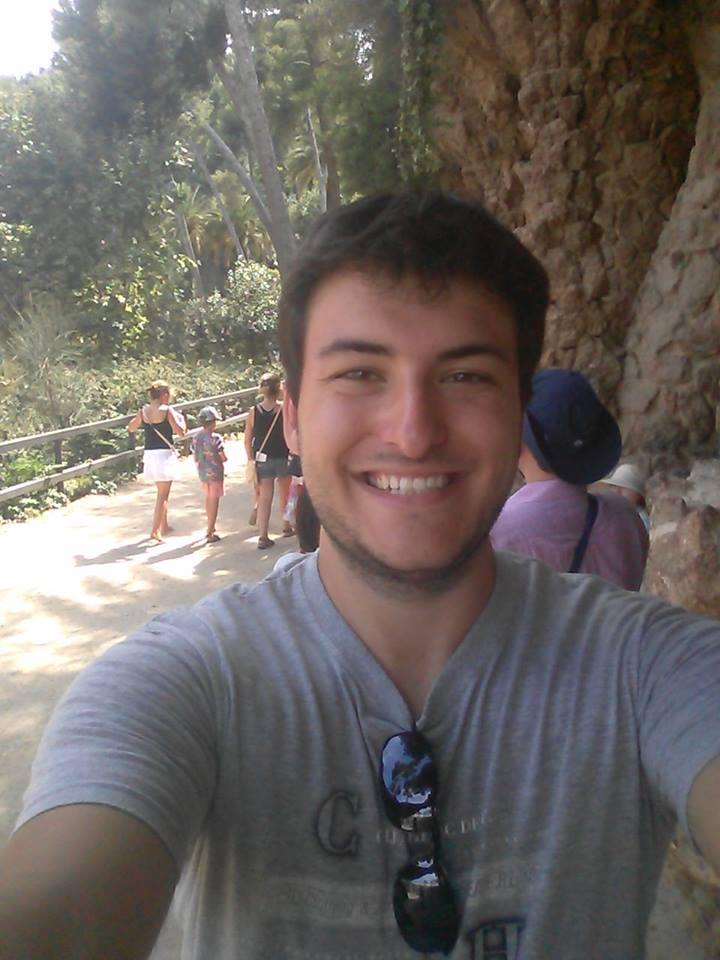
\includegraphics[width=3cm]{../images/alan.jpg}
\item[Christoffer] Studying the Civilingenjör in Computer Science, on the
  Computer Science Master Program at CSC, autonomous systems track
  \\
  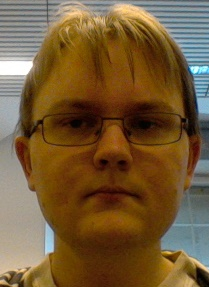
\includegraphics[width=3cm]{../images/christoffer.jpg}
\item[Dmitrij] Is studying computer science here at KTH, 5th year currently.
  Have not attended other universities. Has mostly had courses in math
  (obligatory…), algorithms and programming. Has taken one course in
  image-based classification, so has some (basic) knowledge in computer
  vision.
  \\
  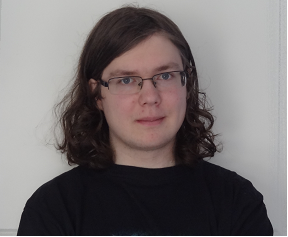
\includegraphics[width=3cm]{../images/dmitrij.jpg}
\item[Michal] Studied BSc in Computer Science at the University of Birmingham in
  the UK, spending one year at Keio University in Tokyo. Now studying Systems,
  Control and Robotics at KTH following the Robotics and Autonomous Systems
  track as an international masters student.
  \\
  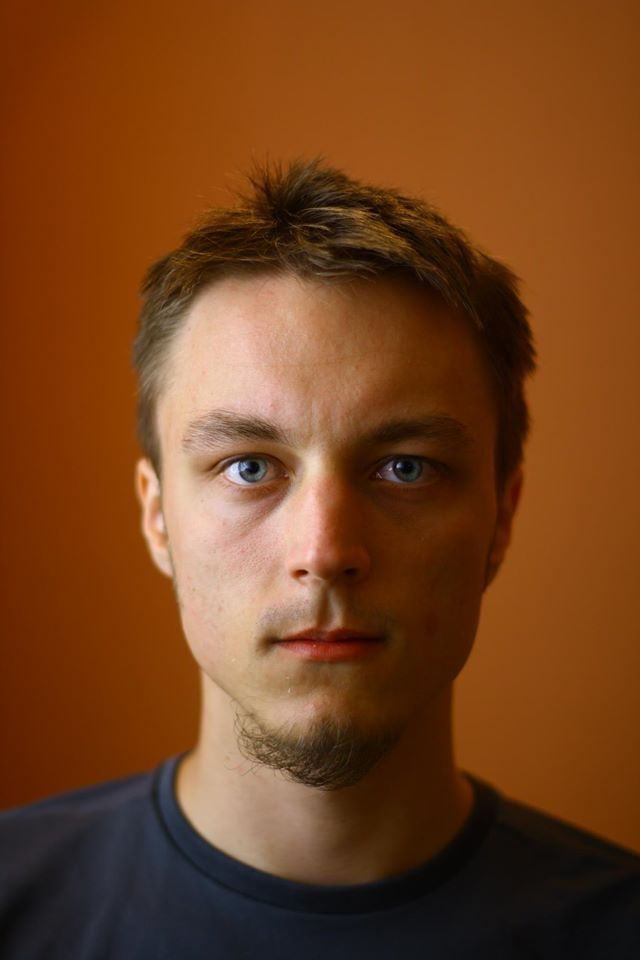
\includegraphics[width=3cm]{../images/michal.jpg}
\item[Yavor] Studied his BSc in Electrical engineering - control and autonomous
  systems at TU Sofia, now studying Systems, Control and Robotics MSc.\\
  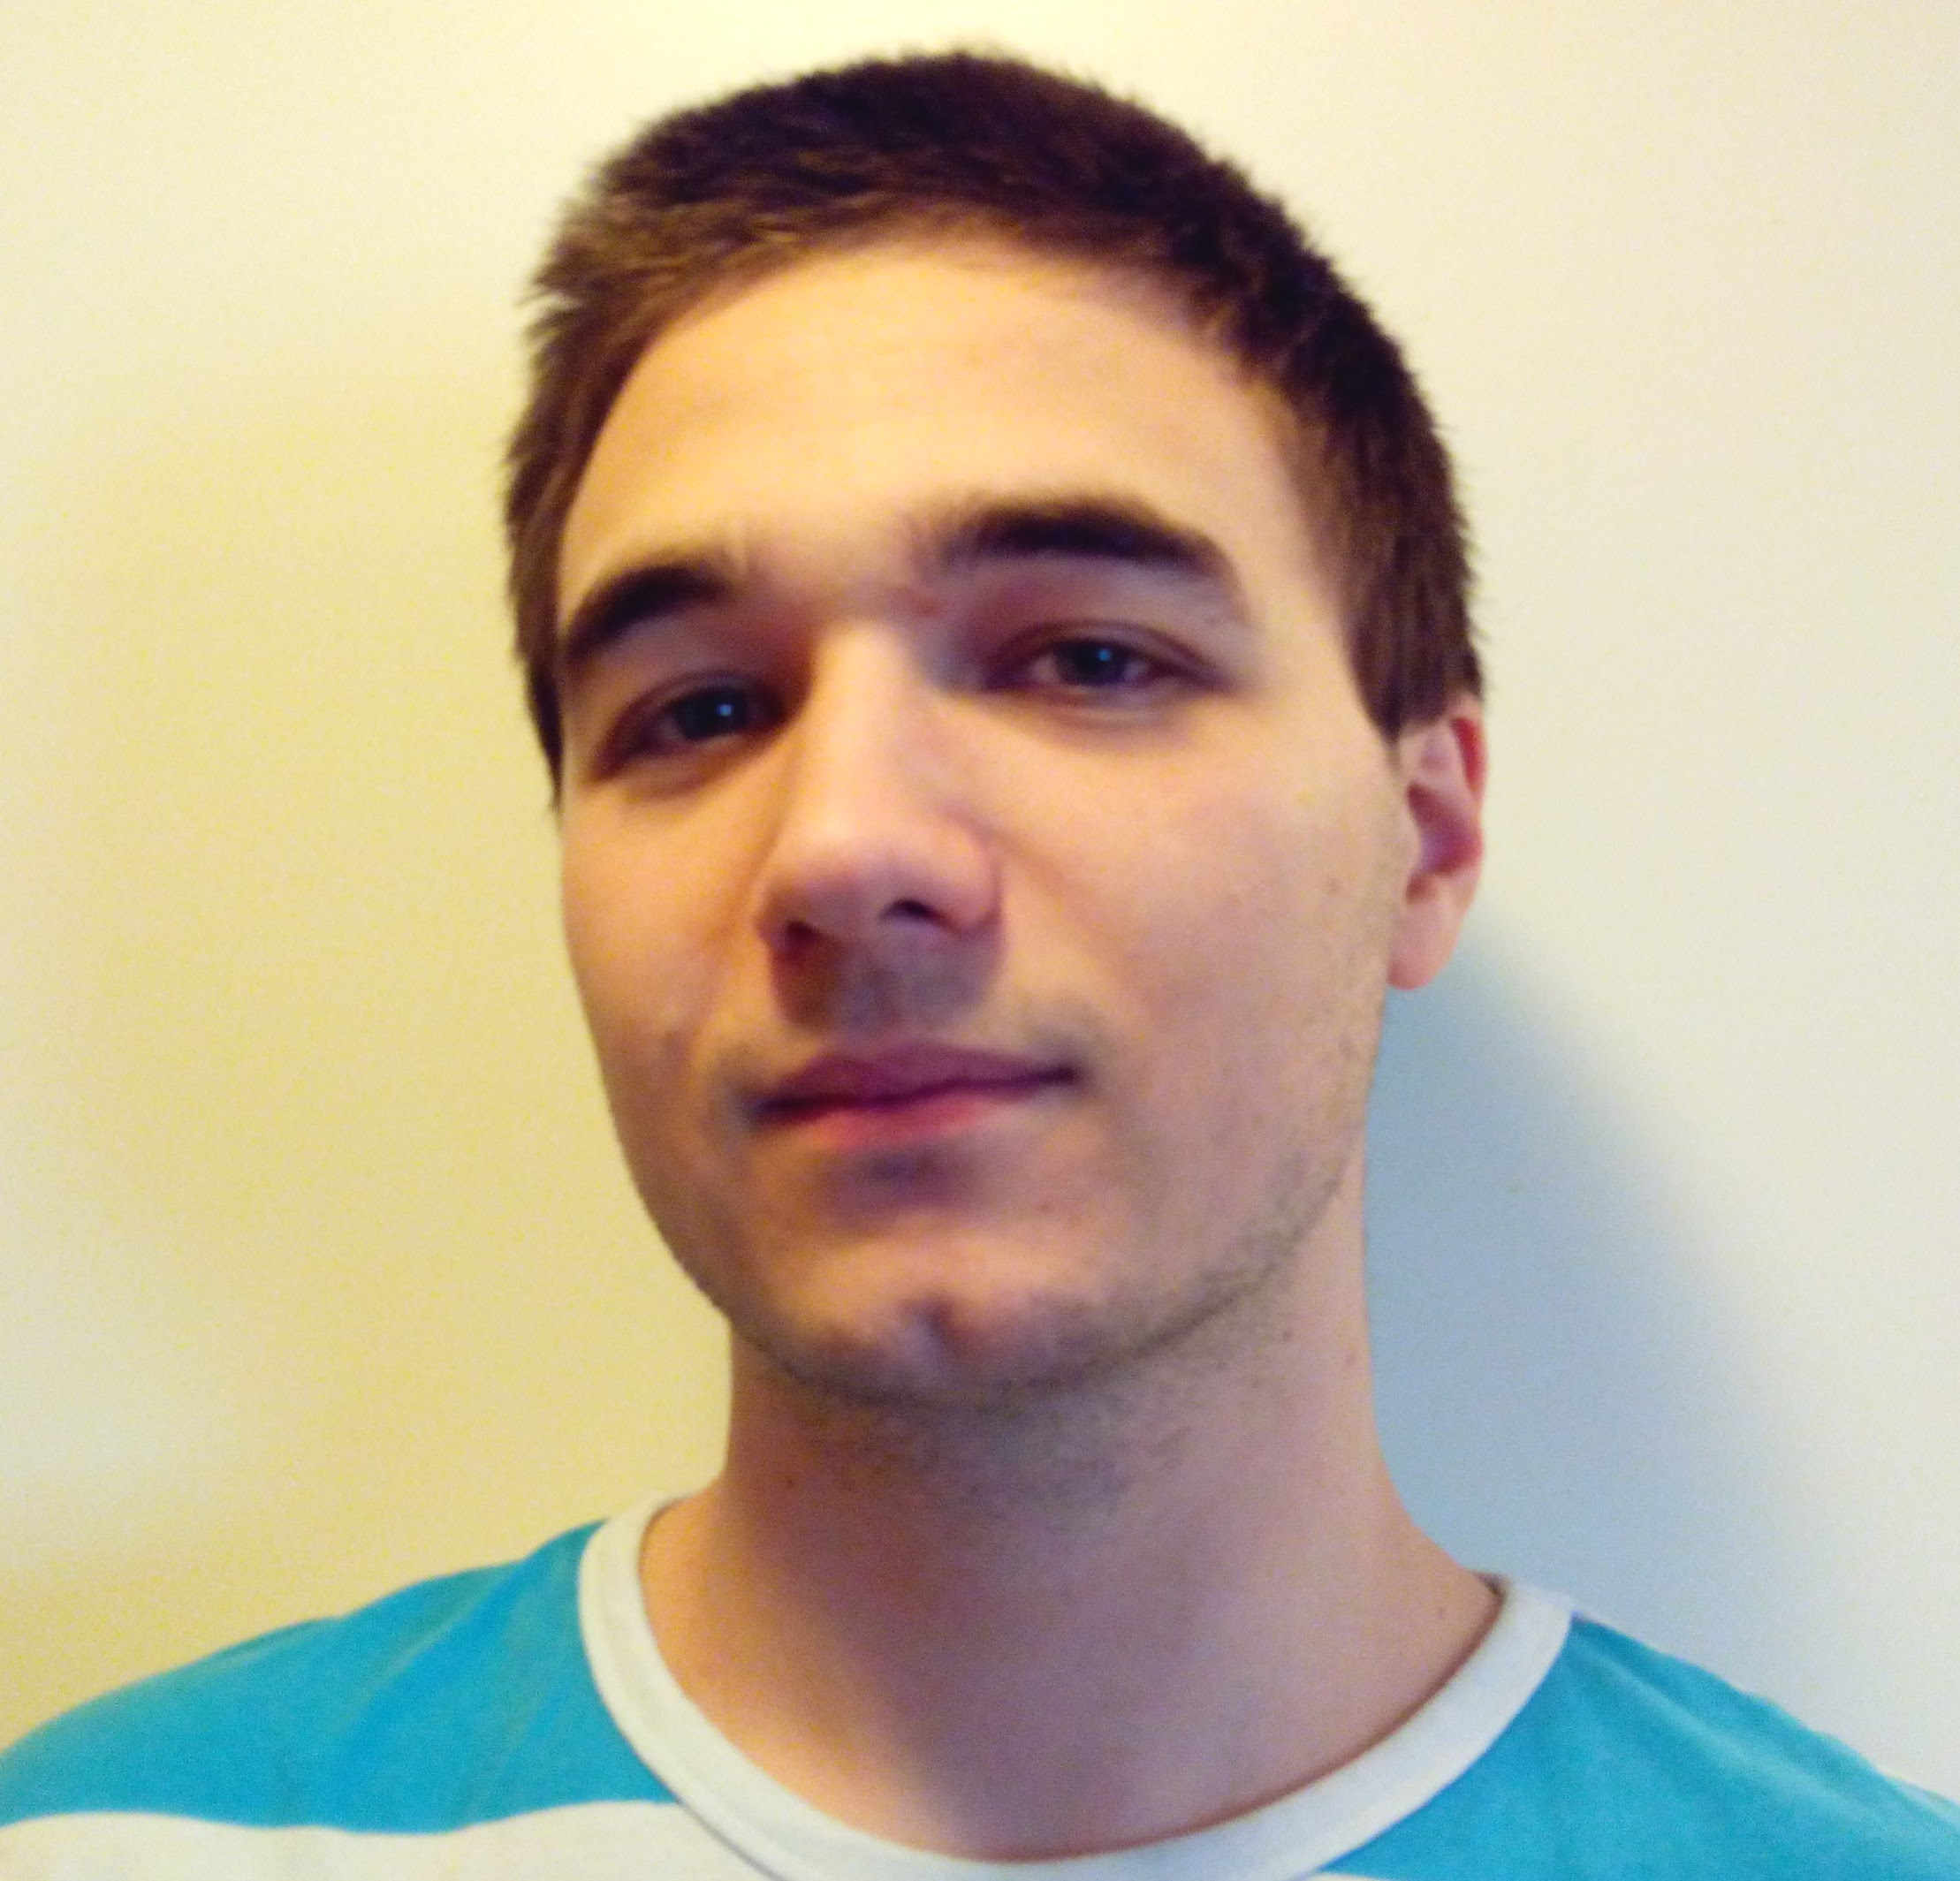
\includegraphics[width=3cm]{../images/yavor.jpg}
\end{description}

\end{document}